% !TEX root = ../my-thesis.tex
\graphicspath{{../cover/}}
% \makeatletter\typeout{\Ginput@path}\makeatother
%
% ------------------------------------  --> cover title page
\begin{titlepage}
	\pdfbookmark[0]{Cover}{Cover}
	\begin{tikzpicture}[remember picture,overlay,node distance=-0.2cm]  
        % Background image     
        % Title & Subtitle 
		\node[above right,
			inner sep=0pt, 
			yshift=-0cm
			] at (current page.south west) (trees) {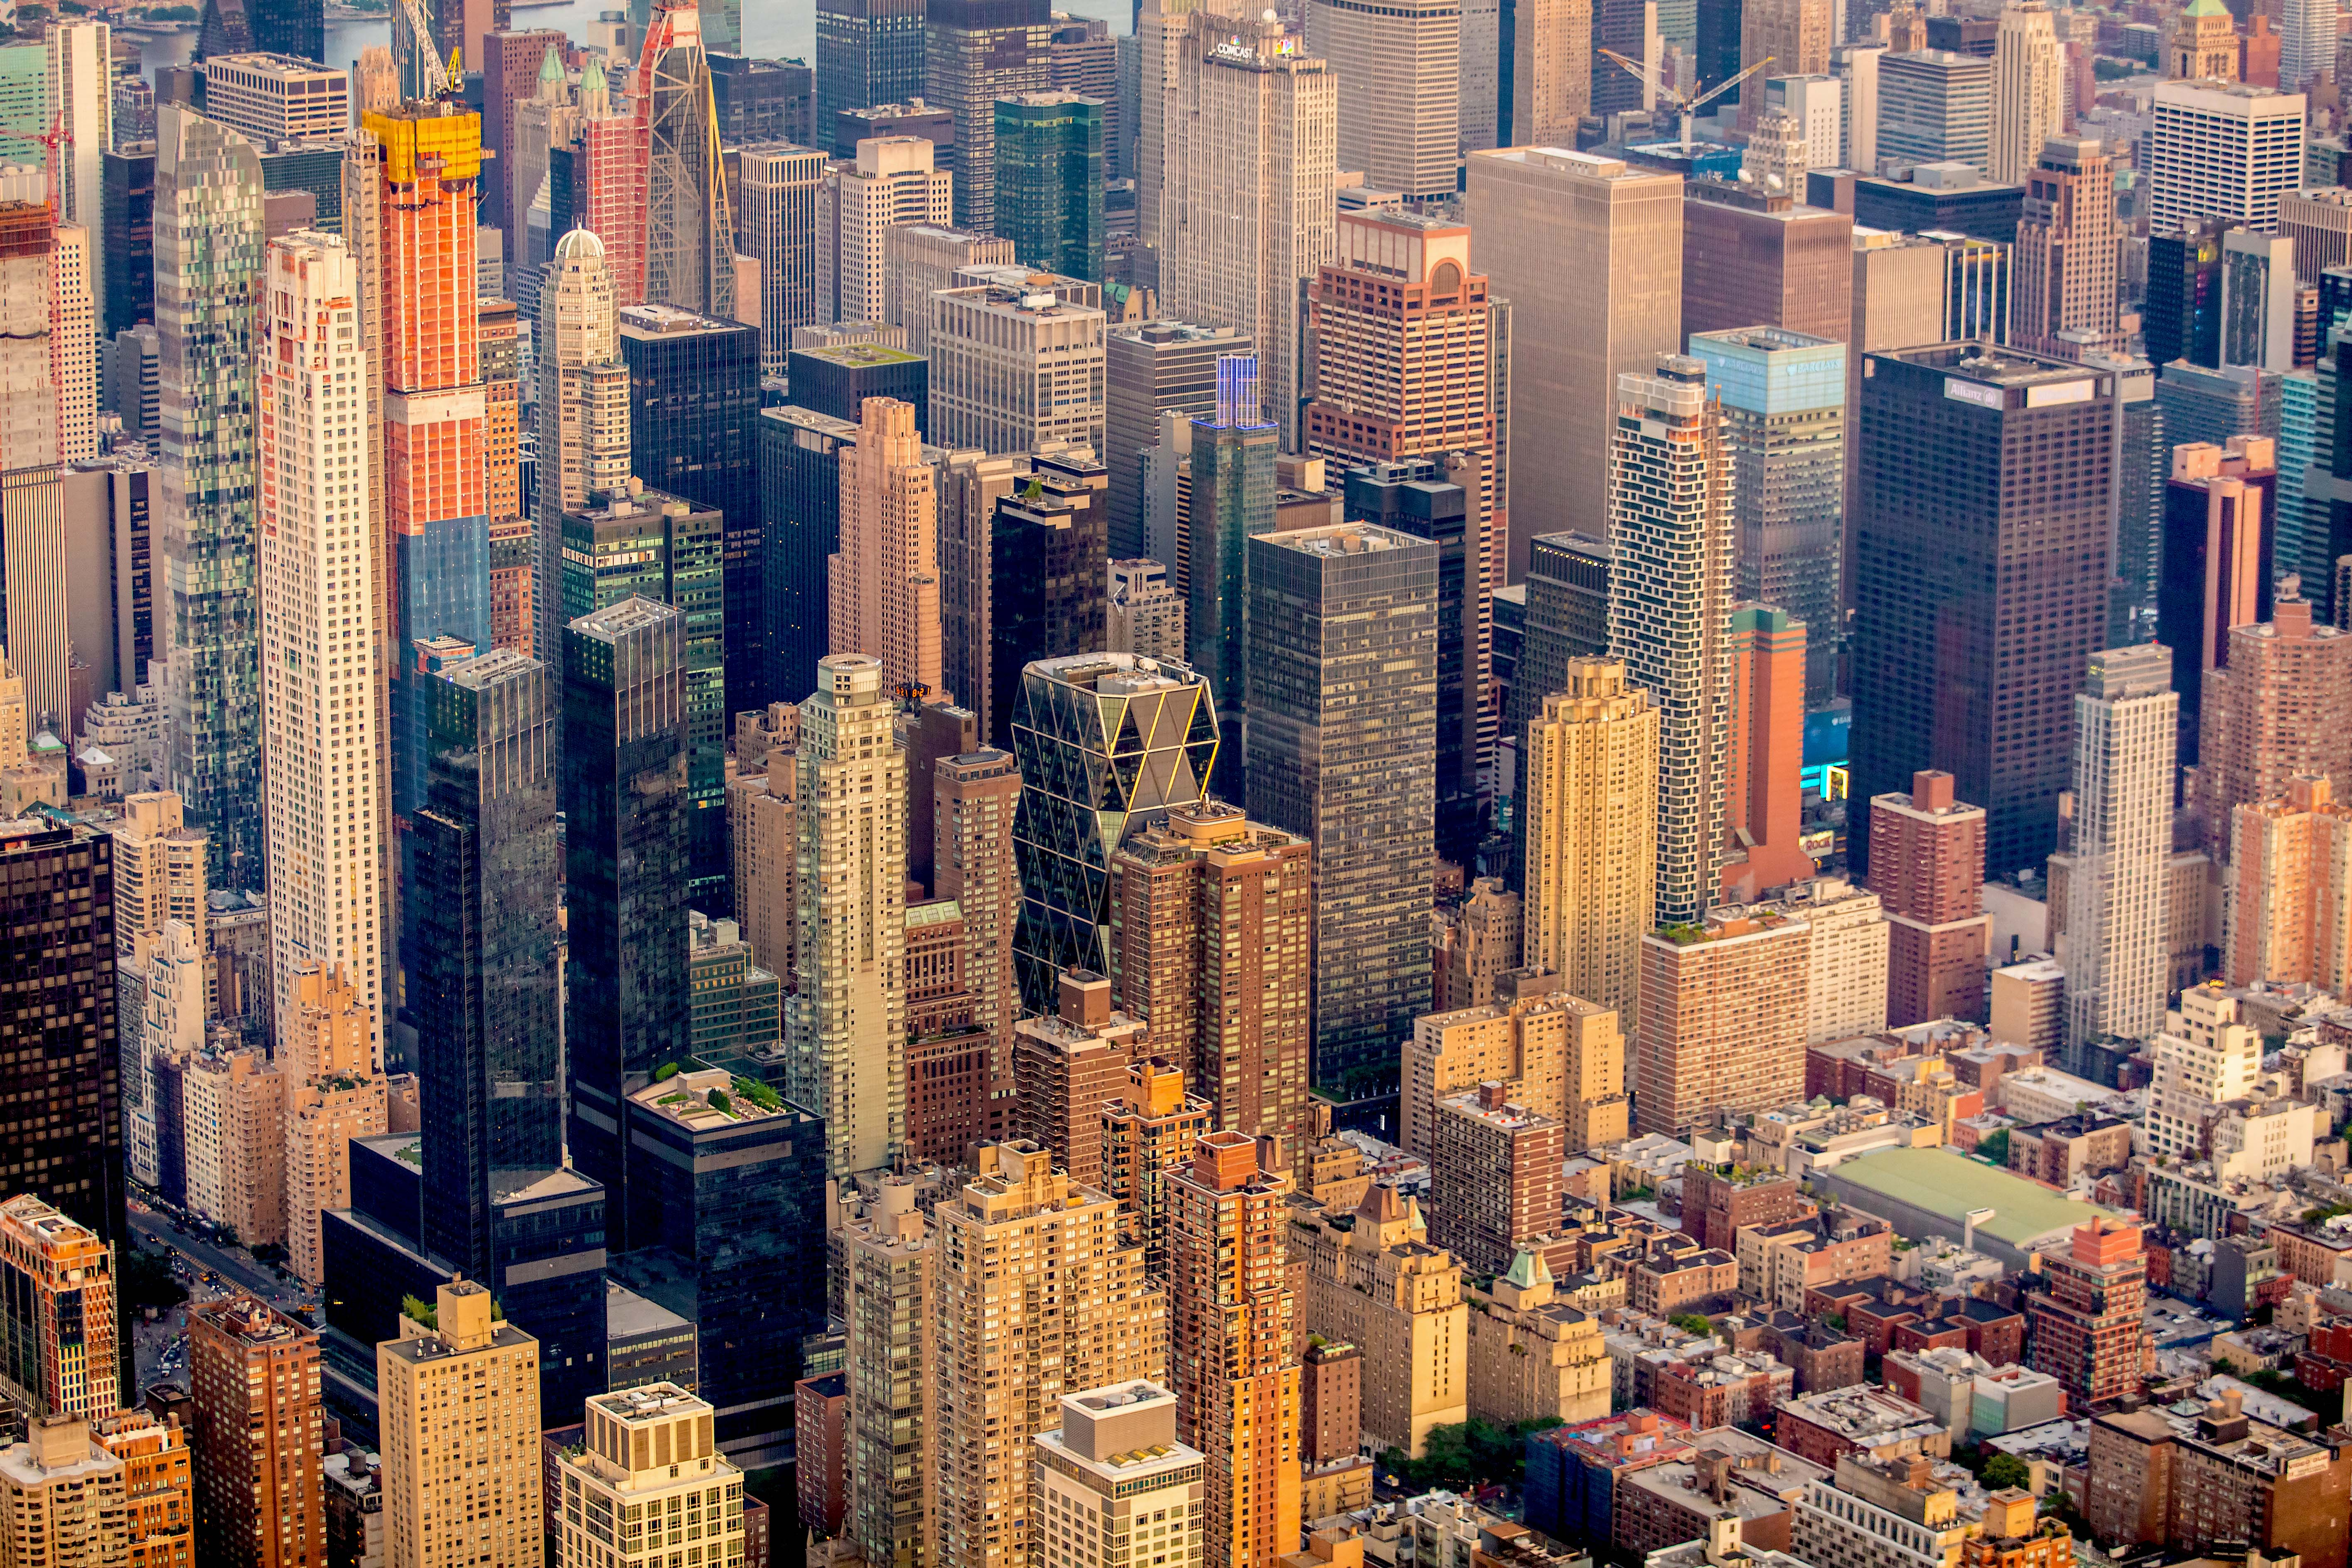
\includegraphics[height=0.5\paperheight]{buildings.jpg}};      
		\node[above = of trees,inner sep=0pt, 
		% yshift=-0.25cm
		]
		{\includegraphics[height=0.5\paperheight]{luca-bravo-A-fubu9QJxE-unsplash.jpg}};     
       
		\node [
            %   below=0.5cm,     
              align=center,     
              text=white,     
              opacity=1,
              text opacity=1,
              rounded corners,     
              inner xsep=15pt,     
              inner ysep=15pt,
			  yshift = -3.5cm,    
            %   minimum width=0.7\textwidth, 
            %   minimum height=0.7\paperheight,
            %   text width=0.6\textwidth,
              ] (title) at (current page.center) {
                \begin{minipage}[b]{\textwidth}
					% \begin{center}
					% \hfill
					% \vfill
					% {\LARGE \color{ctcolortitle}\textbf{\thesisTitle} \\[5mm]}
					\Large{Victor 
					% \color{ctcolortitle}
					\textbf{BOUSSANGE}}\\[0.4cm]
					\Huge{
					% \color{ctcolortitle}
					\textbf{Forward and inverse modelling\\
					of eco-evolutionary dynamics}}\\
					\LARGE{in ecological and economic systems
					}\\[12.3cm]
					\Large{Diss. ETH No. 28804}
					% \flushright
					% \end{center}
                  \end{minipage}
              };  
		% \node[align=center,     
		% 	text=white,     
		% 	opacity=1,
		% 	above left= 2cm of current page.south east,
		% 	xshift=1cm] {
		% 		\Large{Diss. ETH No. 28804}
		% 		};
			% \node[yshift = 0.5cm, 
			% 	%xshift = -3cm, 
			% 	fill=white,
			% 	minimum width=\paperwidth,
			% 	align=center
			% 	% rounded corners
			% 	] at (current page.south) (trees) {{\large Victor \color{ctcolortitle}\textbf{BOUSSANGE}}};      
		 

        % % Author  
        % \node[ below=0.5cm] (author) at (title.south){LaTeX-beamer.com};  
        % % Date 
        % \node[below=0.5cm] (date) at (author.south){\large \today};  
        % Logo
        %  \node [  below right =0.25cm and 0.5cm ] at (current page.north west) {\includegraphics[width=3.5cm]{Beamer-Logo.png} };  
    \end{tikzpicture}
\end{titlepage}



% ------------------------------------  --> main title page
% \begin{titlepage}
% 	\pdfbookmark[0]{Titlepage}{Titlepage}
% 	\tgherosfont
% 	\centering

% 	% \includegraphics[width=6cm]{gfx/Clean-Thesis-Logo} \\[2mm]
% 	% ********************** ADDED by Victor
% 	\noindent
% 	
\includegraphics[viewport=8 8 185 55]{figures/eth_logo_black} \hfill
% 	
\includegraphics[scale=.4]{figures/WSL_sw}\\[4mm]
% 	% **********************

% 	{\Large \thesisUniversity} \\[4mm]
% 	\textsf{\thesisUniversityDepartment} \\
% 	\textsf{\thesisUniversityInstitute} \\
% 	\textsf{\thesisUniversityGroup} \\

% 	\vfill
% 	% {\large \thesisSubject} \\[5mm]
% 	{\LARGE \color{ctcolortitle}\textbf{\thesisTitle} \\[10mm]}
% 	{\Large \thesisName} \\

% 	\vfill
% 	\begin{minipage}[t]{.27\textwidth}
% 		\raggedleft
% 		\textit{1. Reviewer}
% 	\end{minipage}
% 	\hspace*{15pt}
% 	\begin{minipage}[t]{.65\textwidth}
% 		{\Large \thesisFirstReviewer} \\
% 	  	{\small \thesisFirstReviewerDepartment} \\[-1mm]
% 		{\small \thesisFirstReviewerUniversity}
% 	\end{minipage} \\[5mm]
% 	\begin{minipage}[t]{.27\textwidth}
% 		\raggedleft
% 		\textit{2. Reviewer}
% 	\end{minipage}
% 	\hspace*{15pt}
% 	\begin{minipage}[t]{.65\textwidth}
% 		{\Large \thesisSecondReviewer} \\
% 	  	{\small \thesisSecondReviewerDepartment} \\[-1mm]
% 		{\small \thesisSecondReviewerUniversity}
% 	\end{minipage} \\ [5mm]
% 	\begin{minipage}[t]{.27\textwidth}
% 		\raggedleft
% 		\textit{3. Reviewer}
% 	\end{minipage}
% 	\hspace*{15pt}
% 	\begin{minipage}[t]{.65\textwidth}
% 		{\Large \thesisThirdReviewer} \\
% 	  	{\small \thesisThirdReviewerDepartment} \\[-1mm]
% 		{\small \thesisThirdReviewerUniversity}
% 	\end{minipage} \\[10mm]
% 	\begin{minipage}[t]{.27\textwidth}
% 		\raggedleft
% 		\textit{Supervisors}
% 	\end{minipage}
% 	\hspace*{15pt}
% 	\begin{minipage}[t]{.65\textwidth}
% 		\thesisFirstSupervisor
% 	\end{minipage} \\[10mm]

% 	\thesisDate \\

% \end{titlepage}


% ------------------------------------  --> lower title back for single page layout
\hfill
\vfill
{\small
\noindent \textbf{\thesisName} \\
\textit{\thesisTitle} \\
% \thesisSubject, 
\thesisDate \\
% 	Version: \thesisVersion \\
Cover picture: Top: forest in Sorapiss, Dolomites, Italy. Bottom: New York City, USA. @ Luca Bravo / PhotoSpirit\\
The document format is based on the \textit{Clean Thesis} style developed by Ricardo Langner.
% Reviewers: \thesisFirstReviewer\, \thesisSecondReviewer and \thesisThirdReviewer\\
% Supervisors: \thesisFirstSupervisor\ \\[1.5em]
% \textbf{\thesisUniversity} \\
% \textit{\thesisUniversityGroup} \\
% \thesisUniversityInstitute \\
% \thesisUniversityDepartment \\
% \thesisUniversityStreetAddress \\
% \thesisUniversityPostalCode\ and \thesisUniversityCity
}
